\begin{figure*}[htbp]
\centering
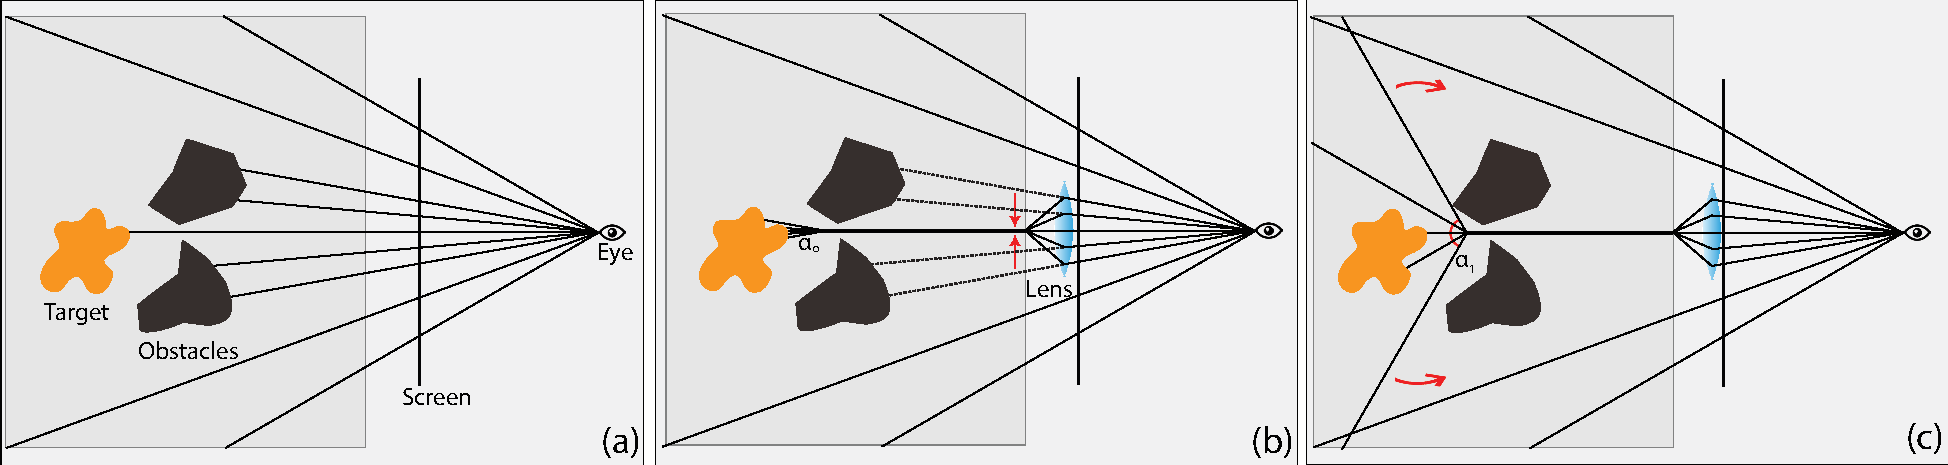
\includegraphics [width=0.8\textwidth]{images/principle.pdf}
\vspace{-0.15cm}
\caption{Principle of the obstruction-free lens. An interesting object is partially hidden by occluders in front of it. (a) Classic raycasting result. (b) Our lens gathers the rays to avoid occluders. Once close to the target, rays follow again their initial paths. However, only a small part of the target is visible. (c) Scattering the rays makes the full target visible.}
\label{f:fisheye}
\vspace{-0.15cm}
\end{figure*}

\section{Principle}
\label{sec:principle}
%
%
Our proposed lens combines the modification of several parameters of a typical DVR rendering of volume data, as follows. Consider the typical DVR algorithm: Given a scalar volume $V \subset \mathbf{R}^3 \rightarrow \mathbf{R}$, each pixel $\mathbf{x} \in I$ in the DVR image $I \subset \mathbf{R}^2$ thereof corresponds to the compositing of sampled data along a ray starting passing through $V$ and ending at $\mathbf{x}$. In classical DVR (\autoref{f:fisheye}-a), such rays are defined by the eye position $\mathbf{e}$ and a viewing-direction unit vector $\mathbf{d} = (\mathbf{x} - \mathbf{e}) / \| \mathbf{x} - \mathbf{e} \|$ pointing from $\mathbf{e}$ to $\mathbf{x}$. Consider next a focus point $\mathbf{f} \in I$ (the \emph{lens center}) and a lens radius $R > 0$. In our proposal, we modify all rays traveling through the disk $D = \{\mathbf{x} \in I | \| \mathbf{x} - \mathbf{f} \| \leq R\}$, or \emph{focus area}, in order to de-occlude, magnify, and emphasize a target object. Our new ray behavior can be divided into three steps: (1) Provide an unobstructed view of the occluded object. This moves closer to the target while avoiding the obstacles by pushing them aside. (2) Set a wide field-of-view (fisheye) to better see the target. (3) Interactively modify various parameters of the lens, lighting, and opacity TF in real time to better explore the target. These steps are detailed next.

\subsection{Creating an unobstructed view}
\label{sec:gathering}
%
The scenario our lens addresses is as follows: Given a volume $V$, users produce a DVR thereof, using whatever suitable TFs and other parameters are applicable. When examining $V$ from various viewpoints, (at least) one viewpoint $(\mathbf{e},\mathbf{d})$ is found from which some intriguing structure is \emph{partially} visible in $I$. We call this structure the \emph{target}. Users next want to quickly and easily unravel the target. For this, we proceed as follows: We first \emph{gather} all rays passing through the lens pixels (focus area $D$) to follow the lens' axis vector $\mathbf{a} = (\mathbf{f} - \mathbf{e}) / \| \mathbf{f} - \mathbf{e} \|$. As explained above, at the location $\mathbf{f}$ of the lens center, we do see an interesting partially occluded target. Hence, by definition, the gathered rays pass \emph{through} occluders to hit this target, otherwise we would not see it. We control gathering by setting the ray direction passing through $\mathbf{x} \in D$ to
%
\begin{equation}
\mathbf{r}(\mathbf{x}) = (1-\alpha) \mathbf{a} + \alpha \mathbf{d},
\label{eqn:gathering}
\end{equation}
%
with $\alpha \in [0,1]$. When $\alpha=0$ (default value), all rays follow the lens axis $\mathbf{a}$, thus, can best pass through obstacles. When $\alpha=1$, rays follow their original classical DVR path. Changing $\alpha$ with the mouse wheel allows one to smoothly navigate between the lens effect, \emph{i.e.} opening up a `hole' in the volume to see the target, and a classical DVR visualizaton of the volume.
%
\subsection{Setting a wide field of view}
\label{sec:scattering}
%
Once the rays pass obstacles (Sec.~\ref{sec:gathering}), we want to \emph{scatter} them so as to best sample the target. Consider that this target is at some depth $t_{target}>0$ within $V$. After the rays pass the occluders, but before they hit the target, \emph{i.e.}, travel past a distance $t_{min} < t_{target}$ through $V$, we deflect (scatter) them so as to best sample the target. For this, we set the parametric position of a ray point to
%
\begin{equation}
\mathbf{p}(\mathbf{x}, t) = \mathbf{r}(\mathbf{x})t + \beta (\mathbf{x}-\mathbf{f})(t-t_{min})
\label{eqn:scattering}
\end{equation}
%
for any pixel $\mathbf{x} \in D$ and any $t \geq t_{min}$. Here, $\beta \geq 0$ controls the ray scattering: Small values magnify a small volume area located close to the ray $\mathbf{r}(\mathbf{x})$; larger values sample more of the volume area behind the lens. Intuitively, this works as if we moved a maginfying lens to a depth $t_{min}$ inside $V$. Summarizing, after the user finds an interesting but partially occluded target using \emph{standard} DVR, the lens squeezes rays to pass between occluders and next fans them out to reveal the target in full detail. The parameter $\beta$ can be adjusted by the user via the mouse scroll wheel while pressing the Shift key (\autoref{f:fisheye}-c).
%
%
\begin{figure}[htbp]
\centering
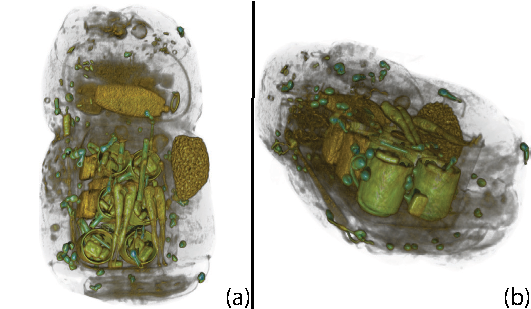
\includegraphics [width=0.4\textwidth]{images/bagage_orientation_bis.pdf}
\caption{A baggage presented under two different perspectives. (a) The baggage is composed by various type of items. the camera is located at the top front of the baggage. (b) The camera is located at the baggage side.}
\label{f:baggage_orientation}
\end{figure}

\subsection{Interactive exploration of the target}
%
We allow users to interactively modify several parameters of the DVR and the lens to achieve a more effective exploration, as follows.

\vspace{0.2cm}
\noindent\textbf{Lens radius:} The lens radius $R$ can be controlled via the mouse wheel, thereby specifying how big is the `hole' to open up in the volume to see the target. The parameters $\alpha$ and $\beta$ controlling respectively the gathering and scattering of rays are controlled by the mouse wheel and modified keys. The value $t_{min}$ controlling the depth from which scattering starts is controlled using the arrow keys.

\vspace{0.2cm}
\noindent\textbf{Lens axis:} Users can rotate the lens axis $\mathbf{a}$ using a virtual trackball activated by the right mouse button. Changing this direction effectively samples the target from all possible viewpoints, thereby allowing the user to look `around' it so as to see its parts which are not visible from the current viewpoint, but \emph{without} having to actually change the viewpoint. This is very important, since changing the viewpoint may bring us to a situation from where the target is completely invisible, so we do not know where precisely to activate the lens any more.

\vspace{0.2cm}
\noindent\textbf{Lighting:} We modify the volumetric Phong lighting parameters to better explore the target, as follows. Let $d(\mathbf{x})$ be the distance from a voxel $\mathbf{x}$ to the target center $\mathbf{e} + \mathbf{a}t_{min}$. Let $\phi$ be the specular term coefficient, set by default to a high value. First, for all voxels $\mathbf{x} \in V$ that project in the lens ($d(\mathbf{x}) \leq R$), we use a specular coefficient $\phi(\mathbf{x}) = \phi (1-d)/R$; all voxels projecting outside the lens lens ($d(\mathbf{x}) > R$) use a value $\phi(\mathbf{x}) = 0$. Hence, voxels close to the lens center appear specular, while voxels outside the lens appear diffuse. Secondly, we allow the user to rotate the light vector using the same trackball mechanism as for the lens axis rotation. These two mechanisms combined realize the effect of a moving flashlight turning around a shiny target. This highlights small-scale details on the target surface, again, without having to change the viewpoint or lens location.

\vspace{0.2cm}
\noindent\textbf{Opacity:} Finally, we modify the opacity transfer function as follows. Let $TF_{o} : \mathbf{R} \rightarrow [0,1]$ be the user-chosen opacity function. Let  $TF^{lens}_{o}$ be an opacity function computed by adding to $TF_{o}$ a Gaussian pulse centered at the average density value $\rho$ in the target. Then, for each voxel $\mathbf{x}$ projecting in the lens, we use an effective transfer function $TF(\mathbf{x}) = TF_{o} d/R + TF^{lens}_{o} (1-d)/R$; for voxels projecting outside the lens, we use $TF_{o}$. The effect is that voxels in a ball or radius $R$ around the target will become less transparent, thus more visible. However, voxels having the same densities but outside this ball will use the default transfer function (which could make them transparent). This allows to have voxels with similar densities either opaque (if they are close to the target, thus interesting) or transparent (if they are \emph{e.g.} in front of the target, thus occluding).


\subsection{Smooth transitions}
\label{continuity}
%
If we apply Eqns.~\ref{eqn:gathering} and~\ref{eqn:scattering} to all rays passing through the lens pixels $D$, and trace all other rays starting at pixels in $I \setminus D$ as usual in DVR, discontinuities will appear at the lens borders. We solve this as follows. Let $\mathbf{p}(\mathbf{x},t)$ be the voxels along a lens ray starting at pixel $\mathbf{x}$, as computed by Eqn.~\ref{eqn:scattering}. Let $\mathbf{p}^{\prime}(\mathbf{x},t)$ be the voxels computed along an straight ray starting at the same pixel, \emph{i.e.}, using $\alpha=1$ and $\beta=0$ in Eqns.~\ref{eqn:gathering} and~\ref{eqn:scattering} respectively. For every value $t$ along every such ray, we then compute the interpolated ray
$\bar{\mathbf{p}}(\mathbf{x},t) = (1-f(d))\mathbf{p}(\mathbf{x},t) + f(d)\mathbf{p}^{\prime}(\mathbf{x},t)$, where $d$ is the unit-normalized distance of $\mathbf{x}$ to the lens axis, and $f : [0,1] \rightarrow [0,1]$ is an interpolation function. Next, we use the rays $\bar{\mathbf{p}}(\mathbf{x},t)$ to compute the DVR by standard composition. This way, rays effectively vary smoothly from their bent versions (close to the lens center) to straight lines (outside the lens). Setting $f(d) = d^2$ keeps the interpolation area close to the lens border, so most of the lens displays the desired fisheye effect.

Separately, we use a slow-in/slow-out animation~\cite{Dragicevic:2011:TDA:1978942.1979233} to introduce the lens effect. When the lens is activated, we vary the values of $\alpha$ and $\beta$ from the defaults ($\alpha=1$, $\beta=0$, \emph{i.e.} straight-line DVR) to their actual user-set values, compute the volume rendering on-the-fly, and display the resulting images. The overall effect resembles opening a hole in the volume. The speed increase at the start of the animation helps one to start tracking the pushed-away occluders; the decreasing speed at the end helps seeing where these occluders actually go. This also gives some semantic to the moving shapes, allowing the human mind to interpret the motion as a magnification of a target, and to keep the focus on visual entities during this transition. When the lens is deactivated, we play back the animation in the opposite sense, which suggests closing the opened hole in the volume.

\section{Implementation}
\label{sec:implem}

Algorithm \ref{alg:propagation} shows a pseudo code of the behavior of our deforming lens


\begin{algorithm}
\SetKwInOut{Input}{Input}
\SetKwInOut{Output}{output}
\SetKwInOut{Parameter}{Parameter}

 \Input{
 $\vec{e}$: the eye position,
 
 $\vec{d}\left(x,y\right)$: the ray direction according to the screen space coordinates of the resulting pixel ($x$ and $y$),
 
 $step$: the sampling distance along the ray.
 
 }
 \KwResult{the pixel color.}
 
 \Parameter{
 $a$: the attraction factor,
 
 $\alpha$: the angle of view.
 }
\BlankLine
 
  $k  \leftarrow $ the normalized distance to the axis of the lens
 $\vec{p}_{near}  \leftarrow \vec{e} + t_{near} \times \vec{d}\left(x,y\right)$ //The initial position  \; 
 $\vec{p}^{0} \leftarrow \vec{p}_{near} $ \; 
 \While{ $ t \le t_{far}$ And $Opacity \le Opacity Threshold  $ }{
 	\If{the current ray is inside the lens}{
    	\If{ $t < t_{target}$ }{
        	$\vec{p}^{1} \leftarrow \vec{p}_{near}\left(x,y\right) + t \times \vec{d}_{target} + a \times \vec{f}_{attraction}$  \;
            \lElse{
        	$\vec{p}^{1} \leftarrow \vec{p}_{target} + \left( t-t_{target} \right) \times \vec{d}_{fishEye}\left( \alpha \right)$
        	}	
        }
               
    $\vec{p} \leftarrow \vec{p}^{0} + f\left(k\right) \times \left( \vec{p}^{1} - \vec{p}^{0} \right) $	\;
     \lElse{
     	 $\vec{p} \leftarrow \vec{p}^{0}$
     }
    }
\emph{Sampling at the position $\vec{p} $ }\;
    
    \emph{Shading the sampled value }\;
    
    \emph{ Compositing the shaded sampling point with the previous values} \;
 
    $t \leftarrow t + step$ \;
    $p^{0} \leftarrow p^{0} + step \times \vec{d}\left(x,y\right)$ \;

}
$color_{final} \leftarrow$ composited colors \;
return $color$
 

\label{alg:propagation}
 \caption{Pseudo code of our lens deformation algorithm}
\end{algorithm}


